
%---------------------------------------------
%	6. Application & Perform of GNN Algorithm
%---------------------------------------------

%\chapter{Application and Performance of GNN Algorithm}\label{chapter-6}

%The main application of the GNN algorithm on the trackML data, the data preparation, what data was exactly used and why, the ML classification algorithm used to build the edge connections. The main results we get from application of this algorithm, the track reconstruction efficiency, the purity metrics, computational performance. Comparison with other algorithms.

%\section{Data Preparation}

%Talk specifically about the TrackML data here and how it was prepared.

%nips-2018-competation
%Data.
%We used the fast (10s per event) and accurate simulation engine ACTS4 [6] to generate the challenge data. It allowed us to generate realistic data emulating a full Silicon LHC detector (see Fig 3), while providing us with the ground truth of particle trajectory membership. Thus, for each event we obtained the “detected” 3D points coordinates (and additional features), and, as ground truth, the list of points associated to each track. There is a one to one relationship between the true 3D points and the reconstructed ones.

%\section{Results}
%\subsection{Performance Evaluation}
%\subsection{Analysis and Optimisation}
%\subsection{Comparison and Outlook}
%\subsection{Execution time}


%---------------------------------------------
%	6. Application & Perform of GNN Algorithm
%---------------------------------------------

\chapter{Application of the GNN Algorithm on the TrackML Model}
\label{chapter-6}

% This chapter focuses on the track finding algorithm development and its application on the publicly available dataset designed for the Kaggle TrackML challenge. The preliminary results related to track reconstruction efficiency and purity metrics are presented and discussed.

%The main application of the GNN algorithm on the trackML data, the data preparation, what data was exactly used and why, the ML classification algorithm used to build the edge connections. The main results we get from application of this algorithm, the track reconstruction efficiency, the purity metrics, computational performance. Comparison with other algorithms.


\section{Data Preparation and Implementation}
%Talk specifically about the TrackML data here and how it was prepared. How the trackml hits are converted into nodes and edges. Close proximity node merging. Checks that are put in place in order to make sure there are no hits that have the same module id (more than 2 hits that are simultaneously in the same module and volume and layer).



\subsection{Constructing Track State Estimates}
- Linear and Parabolic
\subsection{Derivation of Covariance}
\subsection{Moliere Theory of Multiple Scattering}
- Highland formula
\subsection{Determining the Optimal KL Threshold}
\subsection{Linear Extrapolation Model}
\subsection{Parabolic Extrapolation Model}
Mention here that both the linear and parabolic models were used in this instance, where the track state estimate comprised of a 3x1 vector, a, b, tau. The extrapolation and KF update will be different here, different transition Jacobian matrix.



\subsection{Implementation of Kalman Filters}
\label{gnn-kf-implementation}
%\begin{itemize}
%\item emphasis on the use of KFs both in information aggregation stage and in track extraction, both are implemented in different ways, is a useful and unique part to this algorithm
%\item OU process noise
%\end{itemize}




\section{Endcap Results and Performance Evaluation}

% TODO: mention here that the parabolic track state model was used and the joint track state was used, and mention the section here

%nips-2018-competation
%Data.
%We used the fast (10s per event) and accurate simulation engine ACTS4 [6] to generate the challenge data. It allowed us to generate realistic data emulating a full Silicon LHC detector (see Fig 3), while providing us with the ground truth of particle trajectory membership. Thus, for each event we obtained the “detected” 3D points coordinates (and additional features), and, as ground truth, the list of points associated to each track. There is a one to one relationship between the true 3D points and the reconstructed ones.

%\begin{itemize}
%    \item Application on TrackML model, endcap volume only, metrics, performance eval etc, track reconstruction efficiency, track purity and particle purity, comparison with TrackML solutions
%    \item Track reconstruction efficiency, track purity, particle purity
%    \item Performance Evaluation
%    \item execution time?
%\end{itemize}




\section{Outlook}
\subsection{Extension to the Barrel Region}
\subsection{Software Optimisations}
\subsection{Other Approaches}
- Community Detection
- Cellular Automatons

\subsubsection{Community Detection}

%If a subgraph does not meet the criteria to qualify as a good track candidate, a \textit{Community Detection} algorithm \cite{community} is applied in order to further partition the set of nodes. Community Detection is a generalisation of CCA and works by using a distance metric, typically modularity, in order to label nodes as \textit{closely connected}. Modularity is a benefit function that measures the strength of a particular division of a network using the number of edges. A popular modularity maximisation approach is the Louvain method \cite{python_louvain}, which iteratively optimises local communities until global modularity can no longer be improved. An example illustration of a network partition via Community Detection is shown in Figure \ref{fig:community-detection}. Any subgraphs with zero extracted candidates through this procedure are propagated to further stages for additional processing.

%Community Detection: divides nodes into various clusters based on edge structure. It learns from edge weights, and distance and graph objects similarly. 

%\begin{figure}[htbp]
%    \centering
%    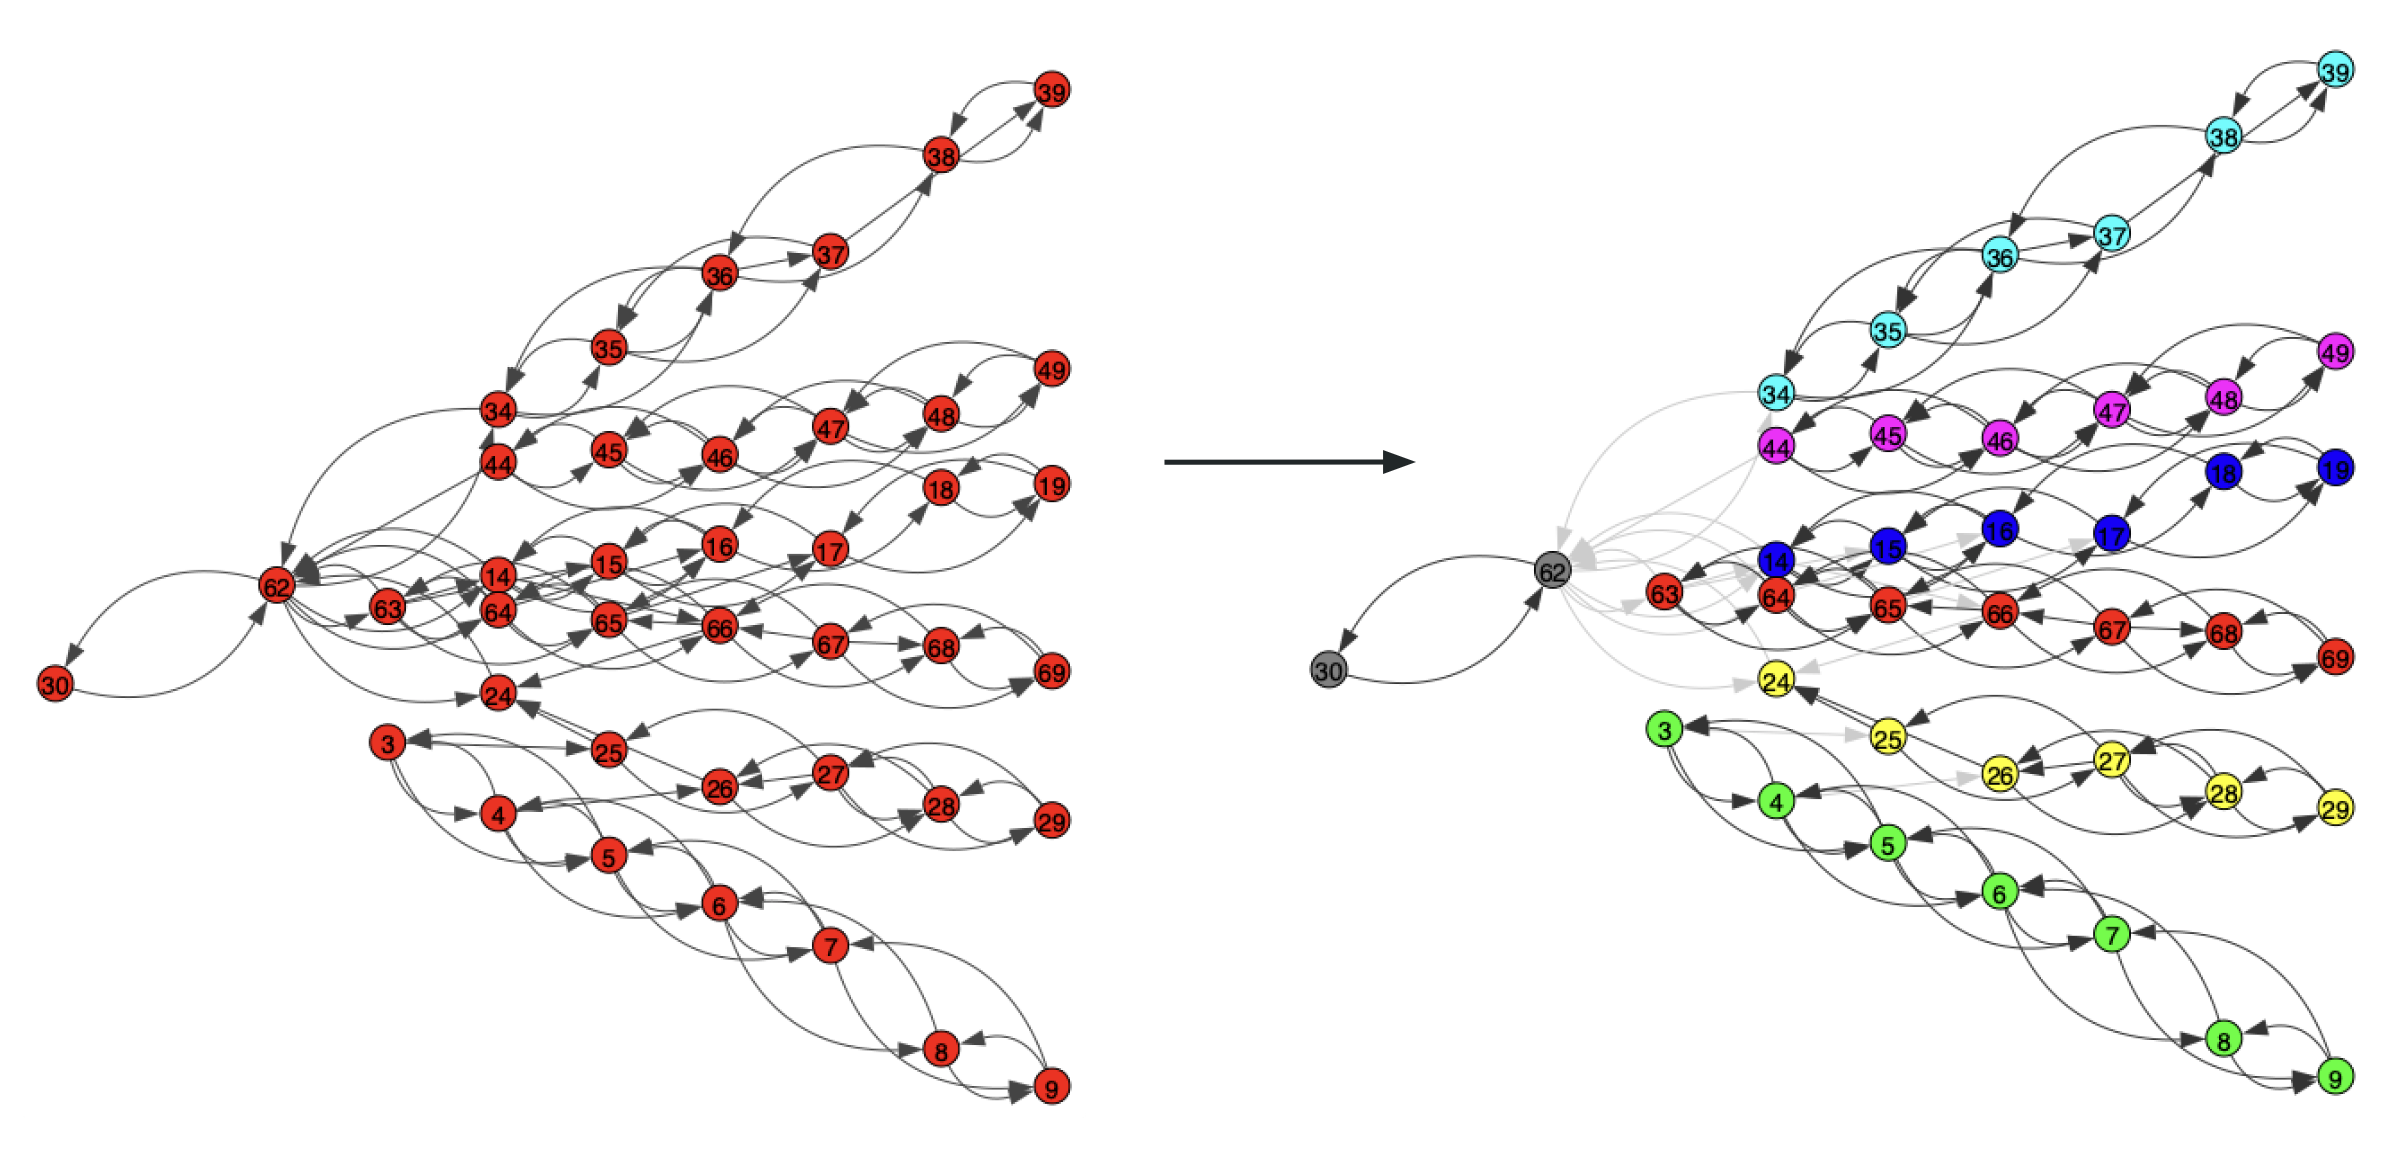
\includegraphics[width=0.98\textwidth]{images/5-gnn-algorithm/community-detection.png}
%    \caption{TODO: caption ....}
%    \label{fig:community-detection}%
%\end{figure}



%\begin{itemize}
%    \item extension to barrel, analysis of results, performance  evaluation, challenges and outlook
%    \item Optimisation - GPU acceleration etc
%\end{itemize}


\section{Conclusions}